\documentclass[10pt,openany]{book}\usepackage[]{graphicx}\usepackage[]{color}
% maxwidth is the original width if it is less than linewidth
% otherwise use linewidth (to make sure the graphics do not exceed the margin)
\makeatletter
\def\maxwidth{ %
  \ifdim\Gin@nat@width>\linewidth
    \linewidth
  \else
    \Gin@nat@width
  \fi
}
\makeatother

\definecolor{fgcolor}{rgb}{0.345, 0.345, 0.345}
\newcommand{\hlnum}[1]{\textcolor[rgb]{0.686,0.059,0.569}{#1}}%
\newcommand{\hlstr}[1]{\textcolor[rgb]{0.192,0.494,0.8}{#1}}%
\newcommand{\hlcom}[1]{\textcolor[rgb]{0.678,0.584,0.686}{\textit{#1}}}%
\newcommand{\hlopt}[1]{\textcolor[rgb]{0,0,0}{#1}}%
\newcommand{\hlstd}[1]{\textcolor[rgb]{0.345,0.345,0.345}{#1}}%
\newcommand{\hlkwa}[1]{\textcolor[rgb]{0.161,0.373,0.58}{\textbf{#1}}}%
\newcommand{\hlkwb}[1]{\textcolor[rgb]{0.69,0.353,0.396}{#1}}%
\newcommand{\hlkwc}[1]{\textcolor[rgb]{0.333,0.667,0.333}{#1}}%
\newcommand{\hlkwd}[1]{\textcolor[rgb]{0.737,0.353,0.396}{\textbf{#1}}}%
\let\hlipl\hlkwb

\usepackage{framed}
\makeatletter
\newenvironment{kframe}{%
 \def\at@end@of@kframe{}%
 \ifinner\ifhmode%
  \def\at@end@of@kframe{\end{minipage}}%
  \begin{minipage}{\columnwidth}%
 \fi\fi%
 \def\FrameCommand##1{\hskip\@totalleftmargin \hskip-\fboxsep
 \colorbox{shadecolor}{##1}\hskip-\fboxsep
     % There is no \\@totalrightmargin, so:
     \hskip-\linewidth \hskip-\@totalleftmargin \hskip\columnwidth}%
 \MakeFramed {\advance\hsize-\width
   \@totalleftmargin\z@ \linewidth\hsize
   \@setminipage}}%
 {\par\unskip\endMakeFramed%
 \at@end@of@kframe}
\makeatother

\definecolor{shadecolor}{rgb}{.97, .97, .97}
\definecolor{messagecolor}{rgb}{0, 0, 0}
\definecolor{warningcolor}{rgb}{1, 0, 1}
\definecolor{errorcolor}{rgb}{1, 0, 0}
\newenvironment{knitrout}{}{} % an empty environment to be redefined in TeX

\usepackage{alltt}

%\input{c:/aaaWork/zGnrlLatex/BookPreamble_HC}   % use for the hard-copy version
\input{c:/aaaWork/zGnrlLatex/BookPreamble}
\hypersetup{pdftitle = MTH107 Notes,bookmarksdepth=0}
\input{c:/aaaWork/zGnrlLatex/JustRPreamble}
\usepackage{animate}
\usepackage{titlesec}
\titlespacing\section{0pt}{12pt plus 4pt minus 2pt}{0pt plus 2pt minus 2pt}
\titlespacing\subsection{-3pt}{12pt plus 4pt minus 2pt}{0pt plus 2pt minus 2pt}
\titlespacing\subsubsection{-3pt}{12pt plus 4pt minus 2pt}{0pt plus 2pt minus 2pt}
\renewcommand{\chaptername}{Module}
\IfFileExists{upquote.sty}{\usepackage{upquote}}{}
\begin{document}




  \frontmatter
    %MAKE MINI TABLE OF CONTENTS for each chapter ----------------------------------
\dominitoc
\setcounter{minitocdepth}{1} %sets the depth to show in chapter TOC -- 0 is chapters, 1 would be sections, etc.

\VerbatimFootnotes  % allows verbatim in footnotes

%TITLE PAGE --------------------------------------------------------------------
\begin{titlepage}
\begin{center}

% Upper part of the page
\textsc{\LARGE Northland College}\\[0.5cm]
\textsc{\Large MTH107 -- Statistical Analysis and Interpretation}\\[1.5cm]

\HRuleW \\
\HRule \\[1cm]
{ \huge \bfseries Introduction to Statistical Analysis and Interpretation}\\[1cm]
\HRule \\
\HRuleW \\[1.5cm]

% Author and supervisor
\begin{minipage}{0.4\textwidth}
\begin{flushleft}
%  \Large \emph{Author:}\\ Dr. Derek H. Ogle
  \Large \emph{Instructors:}\\Dr. Derek H. Ogle \\ Jodi Supanich
\end{flushleft}
\end{minipage}
\begin{minipage}{0.4\textwidth}
\begin{flushright}
  \Large \emph{Department:} \\ Mathematical Sciences
%  \Large \emph{Department:} \\ Mathematical Sciences \\ Mathematical Sciences
\end{flushright}
\end{minipage}

\vfill

% Bottom of the page
%\includegraphics[width=4in]{Title.JPG} \\[2.5cm]
{\Large \today}

\end{center}

\end{titlepage}

% The material in the Preface_OLD.tex file was between here
% and here

%TABLE OF CONTENTS ---------------------------------------------------------------------------------------------------
\setcounter{tocdepth}{0} %sets the depth to show in TOC -- 0 is chapters, 1 would be sections, etc.

%modify what the parts look like
\renewcommand{\cftpartfont}{\scshape}                          %changes to small caps

%modify what the chapters look like
\setlength{\cftchapindent}{1.5em}                              %indent the chapters
\setlength{\cftbeforechapskip}{0.4em}                          %set the space between chapters -- reduce to 0.2 if depth is set to 0

%modify what the sections look like
\setlength{\cftsecindent}{3.8em}                               %indent the sections --- doesn't seem to work
\setlength{\cftbeforesecskip}{0.2em}                           %set the space between sections

\newpage                                                       %need this so that the TOC will start on its own page
\tableofcontents                                               %build the table of contents

%SETTING FOR LEAVING FRONT MATTER AND GOING TO MAIN DOCUMENT ---------------------------------------------------------
\addtocontents{toc}{\setlength{\cftbeforepartskip}{1.5em}}     %increase distance before parts in the main TOC
\addtocontents{toc}{\cftpagenumbersoff{part}}                  %so page numbers won't appear for parts in the main TOC


  \mainmatter










\chapter{Linear Regression}  \label{chap:Regress}

\minitoc
\vspace{48pt}

\lettrine{L}{inear regression analysis is used to model the relationship} between two quantitative variables for two related purposes -- (i) explaining variability in the response variable and (ii) predicting future values of the response variable. Examples include predicting future sales of a product from its price, family expenditures on recreation from family income, an animal's food consumption in relation to ambient temperature, and a person's score on a German assessment test based on how many years the person studied German.

Exact predictions cannot be made because of natural variability. For example, two people with the same intake of mercury (from consumption of fish) will likely not have the same level of mercury in their blood stream. Thus, the best that can be accomplished is to predict the average or expected value for a person with a particular intake value. This is accomplished by finding the line that best ``fits'' the points on a scatterplot of the data and using that line to make predictions. Finding and using the ``best-fit'' line is the topic of this module.


\section{Response and Explanatory Variables}
Recall from \sectref{sect:RespExplan1} that the response (or dependent) variable is the variable to be predicted or explained and the explanatory (or independent) variable is the variable that will help do the predicting or explaining. In the examples mentioned above, future sales, family expenditures on recreation, the animal's food consumption, and score on the assessment test are response variables and product price, family income, temperature, and years studying German are explanatory variables, respectively. The response variable is on the y-axis and the explanatory variable is on the x-axis of scatterplots.


\section{Slope and Intercept}
The equation of a line is commonly expressed as,
  \[ y = mx + b  \]
where both $x$ and $y$ are variables, $m$ represents the slope of the line, and $b$ represents the y-intercept.\footnote{Hereafter, simply called the ``intercept.''}  It is important that you can look at the equation of a line and identify the response variable, explanatory variable, slope, and intercept. The response variable will always appear on the left side of the equation by itself. The explanatory variable (e.g., $x$) will be on the right side of the equation and will be multiplied by the slope. The value or symbol by itself on the right side of the equation is the intercept. For example, in
\[ blood = 3.501 + 0.579intake \]
\var{blood} is the response variable, \var{intake} is the explanatory variable, $0.579$ is the slope (it is multiplied by the explanatory variable), and $3.501$ is the intercept (it is on the right side and not multiplied by anything). The same conclusions would be made if the equation had been written as
  \[ blood = 0.579intake+3.501 \]

\warn{In the equation of a line, the slope is always multiplied by the explanatory variable and the intercept is always by itself.}

In addition to being able to identify the slope and intercept of a line you also need to be able to interpret these values. Most students define the slope as ``rise over run'' and the intercept as ``where the line crosses the y-axis.''  These ``definitions'' are loose geometric representations. For our purposes, the slope and intercept must be more strictly defined.

To define the slope, first think of ``plugging'' two values of intake into the equation discussed above. For example, if $intake=100$, then $blood=3.501+0.579*100$=61.40 and if $intake$ is one unit larger at $101$, then $blood=3.501+0.579*101$=61.98.\footnote{For simplicity of exposition, the actual units are not used in this discussion. However, ``units'' would usually be replaced with the actual units used for the measurements.} The difference between these two values is 61.98-61.40=$0.579$, which is the same as the slope. Thus, the slope is the change in value of the response variable FOR A SINGLE UNIT CHANGE in the value of the explanatory variable \figrefp{fig:SlopeInt}. That is, mercury in the blood changes 0.579 units FOR A SINGLE UNIT CHANGE in mercury intake. So, if an individual increases mercury intake by one unit, then mercury in the blood will increase by 0.579 units, ON AVERAGE. Alternatively, if one individual has one more unit of mercury intake than another individual, then the first individual will have 0.579 more units of mercury in their blood, ON AVERAGE.

\begin{knitrout}
\definecolor{shadecolor}{rgb}{0.922, 0.922, 0.922}\color{fgcolor}\begin{figure}[hbtp]

{\centering 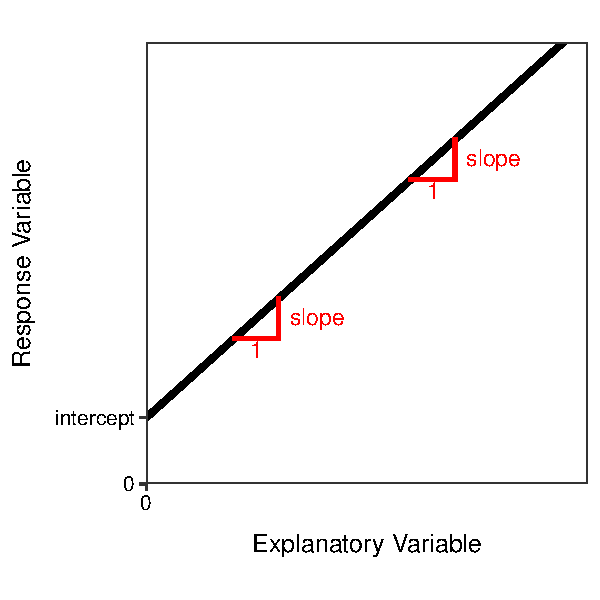
\includegraphics[width=.4\linewidth]{Figs/SlopeInt-1} 

}

\caption[Schematic representation of the meaning of the intercept and slope in a linear equation]{Schematic representation of the meaning of the intercept and slope in a linear equation.}\label{fig:SlopeInt}
\end{figure}


\end{knitrout}

To define the intercept, first ``plug'' $intake=0$ into the equation discussed above; i.e., $blood=3.501+0.579*0$ = $3.501$. Thus, the intercept is the value of the response variable when the explanatory variable is equal to zero \figrefp{fig:SlopeInt}. In this example, the AVERAGE mercury in the blood for an individual with no mercury intake is 3.501. Many times, as is true with this example, the interpretation of the intercept will be nonsensical. This is because $x=0$ will likely be outside the range of the data collected and, perhaps, outside the range of possible data that could be collected.

The equation of the line is a model for the relationship depicted in a scatterplot. Thus, the interpretations for the slope and intercept represent the \textit{average} change or the \textit{average} response variable. Thus, whenever a slope or intercept is being interpreted it must be noted that the result is an \textit{average} or \textit{on average}.


\section{Predictions}
Once a best-fit line has been identified (criteria for doing so is discussed in \sectref{sect:BestFitLine}), the equation of the line can be used to predict the average value of the response variable for individuals with a particular value of the explanatory variable. For example, the best-fit line for the mercury data shown in \figref{fig:HGscat} is
  \[ blood = 3.501 + 0.579*intake \]
Thus, the predicated average level of mercury in the blood for an individual that consumed 240 ug HG/day is found with
  \[ blood = 3.501 + 0.579*240 = 142.461 \]
Similarly, the predicted average level of mercury in the blood for an individual that consumed 575 ug HG/day is found with
  \[ blood = 3.501 + 0.579*575 = 336.426 \]
A prediction may be visualized by finding the value of the explanatory variable on the x-axis, drawing a vertical line until the best-fit line is reached, and then drawing a horizontal line over to the y-axis where the value of the response variable is read \figrefp{fig:HGpredict}.

\begin{knitrout}
\definecolor{shadecolor}{rgb}{0.922, 0.922, 0.922}\color{fgcolor}\begin{figure}[hbtp]

{\centering 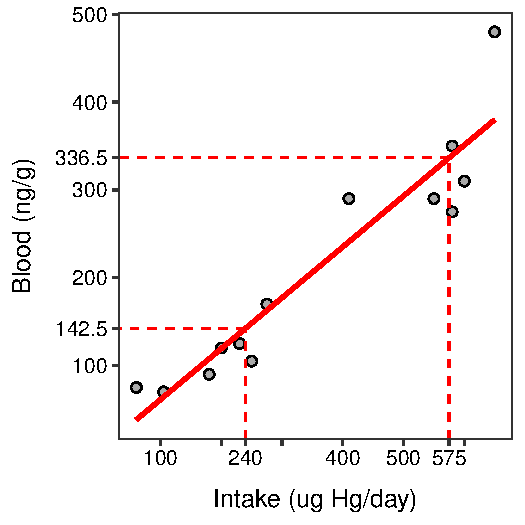
\includegraphics[width=.4\linewidth]{Figs/HGpredict-1} 

}

\caption[Scatterplot between the intake of mercury in fish and the mercury in the blood stream of individuals with superimposed best-fit regression line illustrating predictions for two values of mercury intake]{Scatterplot between the intake of mercury in fish and the mercury in the blood stream of individuals with superimposed best-fit regression line illustrating predictions for two values of mercury intake.}\label{fig:HGpredict}
\end{figure}


\end{knitrout}

\vspace{12pt} %because it was gobbled up
When predicting values of the response variable, it is important to not extrapolate beyond the range of the data. In other words, predictions with values outside the range of observed values of the explanatory variable should be made cautiously (if at all). An excellent example would be to consider height ``data'' collected during the early parts of a human's life (say the first ten years). During these early years there is likely a good fit between height (the response variable) and age. However, using this relationship to predict an individual's height at age 40 would likely result in a ridiculous answer (e.g., over ten feet). The problem here is that the linear relationship only holds for the observed data (i.e., the first ten years of life); it is not known if the same linear relationship exists outside that range of years. In fact, with human heights, it is generally known that growth first slows, eventually quits, and may, at very old ages, actually decline. Thus, the linear relationship found early in life does not hold for later years. Critical mistakes can be made when using a linear relationship to extrapolate outside the range of the data.

\section{Residuals}
The predicted value is a ``best-guess'' for an individual based on the best-fit line. The actual value for any individual is likely to be different from this predicted value. The \textbf{residual} is a measure of how ``far off'' the prediction is from what is actually observed. Specifically, the residual for an individual is found by subtracting the predicted value (given the individual's observed value of the explanatory variable) from the individual's observed value of the response variable, or
  \[ \text{residual}=\text{observed response}-\text{predicted response} \]

For example, consider an individual that has an observed intake of 650 and an observed level of mercury in the blood of 480. As shown in the previous section, the predicted level of mercury in the blood for this individual is
  \[ blood = 3.501 + 0.579*650 = 379.851 \]

The residual for this individual is then $480-379.851$ = $100.149$. This positive residual indicates that the observed value is approximately 100 units GREATER than the average for individuals with an intake of 650.\footnote{In other words, the observed value is ``above'' the line.}  As a second example, consider an individual with an observed intake of 250 and an observed level of mercury in the blood of 105. The predicted value for this individual is
  \[ blood = 3.501 + 0.579*250 = 148.251 \]

and the residual is $105-148.251$ = $-43.251$. This negative residual indicates that the observed value is approximately 43 units LESS than the average for individuals with an intake of 250.

Visually, a residual is the vertical distance between an individual's point and the best-fit line \figrefp{fig:HGresidual}.

\begin{knitrout}
\definecolor{shadecolor}{rgb}{0.922, 0.922, 0.922}\color{fgcolor}\begin{figure}[hbtp]

{\centering 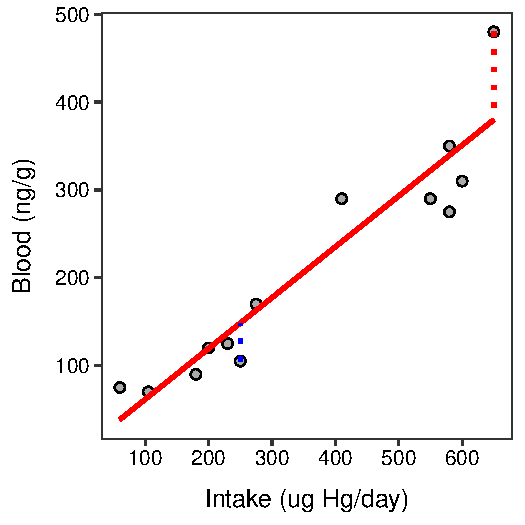
\includegraphics[width=.4\linewidth]{Figs/HGresidual-1} 

}

\caption[Scatterplot between the intake of mercury in fish and the mercury in the blood stream of individuals with superimposed best-fit regression line illustrating the residuals for the two individuals discussed in the main text]{Scatterplot between the intake of mercury in fish and the mercury in the blood stream of individuals with superimposed best-fit regression line illustrating the residuals for the two individuals discussed in the main text.}\label{fig:HGresidual}
\end{figure}


\end{knitrout}

\section{Best-fit Criteria}\label{sect:BestFitLine}
An infinite number of lines can be placed on a graph, but many of those lines do not adequately describe the data. In contrast, many of the lines will appear, to our eye, to adequately describe the data. So, how does one find THE best-fit line from all possible lines. The \textbf{least-squares} method described below provides a quantifiable and objective measure of which line best ``fits'' the data.

Residuals are a measure of how far an individual is from a candidate best-fit line. Residuals computed from all individuals in a data set measure how far all individuals are from the candidate best-fit line. Thus, the residuals for all individuals can be used to identify the best-fit line.

The residual sum-of-squares (RSS) is the sum of all squared residuals. The least-squares criterion says that the ``best-fit'' line is the one line out of all possible lines that has the minimum RSS \figrefp{fig:RSSanim}.

\begin{knitrout}
\definecolor{shadecolor}{rgb}{0.922, 0.922, 0.922}\color{fgcolor}









































































\begin{figure}[hbtp]

{\centering \animategraphics[width=.8\linewidth,controls,palindrome,autoplay]{1}{Figs/RSSanim-}{1}{75}

}

\caption[An animation illustrating how the residual sum-of-squares (RSS) for a series of candidate lines (red lines) is minimized at the best-fit line (green line)]{An animation illustrating how the residual sum-of-squares (RSS) for a series of candidate lines (red lines) is minimized at the best-fit line (green line).}\label{fig:RSSanim}
\end{figure}


\end{knitrout}

\vspace{12pt} %because it got gobbled up

The discussion thusfar implies that all possible lines must be ``fit'' to the data and the one with the minimum RSS is chosen as the ``best-fit'' line. As there are an infinite number of possible lines, this would be impossible to do. Theoretical statisticians have shown that the application of the least-squares criterion always produces a best-fit line with a slope given by
  \[ slope = r\frac{s_{y}}{s_{x}}  \]

and an intercept given by
  \[ intercept = \bar{y}-slope*\bar{x}   \]

where $\bar{x}$ and $s_{x}$ are the sample mean and standard deviation of the explanatory variable, $\bar{y}$ and $s_{y}$ are the sample mean and standard deviation of the response variable, and $r$ is the sample correlation coefficient between the two variables. Thus, using these formulas finds the slope and intercept for the line, out of all possible lines, that minimizes the RSS.


\section{Assumptions}\label{sect:RegAssumptions}
The least-squares method for finding the best-fit line only works appropriately if each of the following five assumptions about the data has been met.

\begin{Enumerate}
  \item A line describes the data (i.e., a linear form).
  \item Homoscedasticity.
  \item Normally distributed residuals at a given x.
  \item Independent residuals at a given x.
  \item The explanatory variable is measured without error.
\end{Enumerate}

While all five assumptions of linear regression are important, only the first two are vital when the best-fit line is being used primarily as a descriptive model for data.\footnote{In contrast to using the model to make inferences about a population model.}  Description is the primary goal of linear regression used in this course and, thus, only the first two assumptions are considered further.

The linearity assumption appears obvious -- if a line does not represent the data, then don't try to fit a line to it!  Violations of this assumption are evident by a non-linear or curving form in the scatterplot.

The homoscedasticity assumption states that the variability about the line is the same for all values of the explanatory variable. In other words, the dispersion of the data around the line must be the same along the entire line. Violations of this assumption generally present as a ``funnel-shaped'' dispersion of points from left-to-right on a scatterplot.

Violations of these assumptions are often evident on a ``fitted-line plot'', which is a scatterplot with the best-fit line superimposed \figrefp{fig:ResidPlotEx}.\footnote{Residual plots, not discussed in this text, are another plot that often times is used to better assess assumption violations.} If the points look more-or-less like random scatter around the best-fit line, then neither the linearity nor the homoscedasticity assumption has been violated. A violation of one of these assumptions should be obvious on the scatterplot. In other words, there should be a clear curvature or funneling on the plot.

\begin{knitrout}
\definecolor{shadecolor}{rgb}{0.922, 0.922, 0.922}\color{fgcolor}\begin{figure}[hbtp]

{\centering 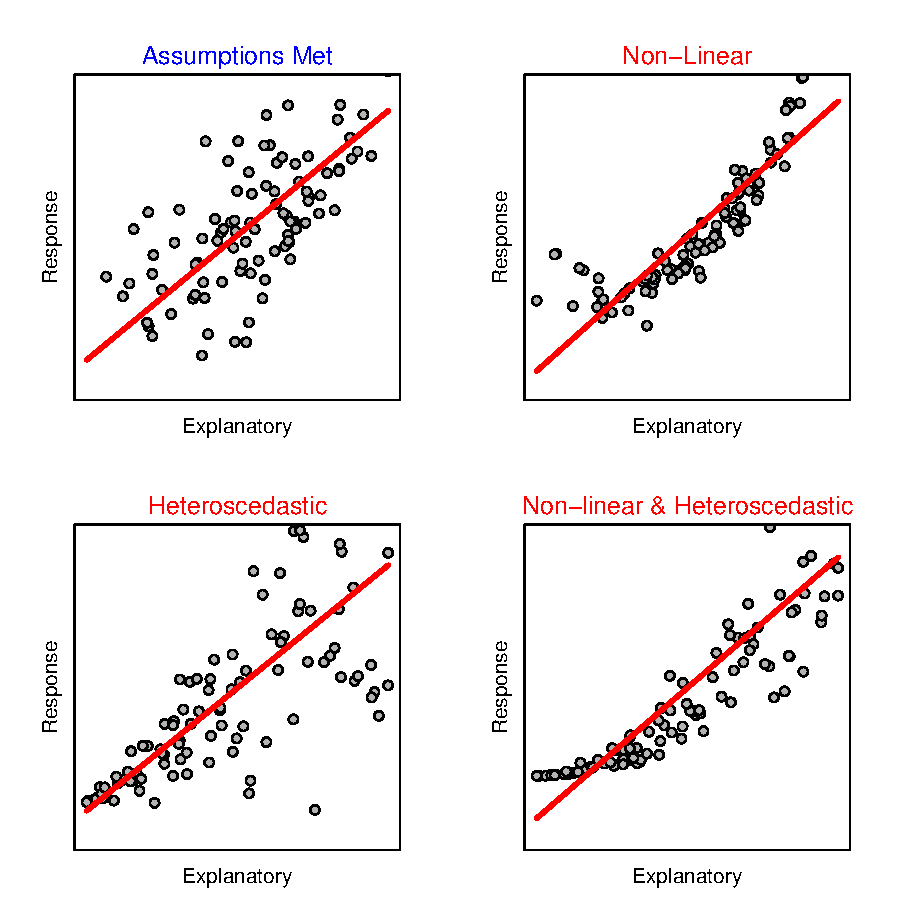
\includegraphics[width=.75\linewidth]{Figs/ResidPlotEx-1} 

}

\caption[Fitted-line plots illustrating when the regression assumptions are met (upper-left) and three common assumption violations]{Fitted-line plots illustrating when the regression assumptions are met (upper-left) and three common assumption violations.}\label{fig:ResidPlotEx}
\end{figure}


\end{knitrout}

In this course, if an assumption has been violated, then one should not continue to interpret the linear regression. However, in many instances, an assumption violation can be ``corrected'' by transforming one or both variables to a different scale. Transformations are not discussed in this course.

\warn{If the regression assumptions are not met, then the regression results should not be interpreted.}


\section{Coefficient of Determination}
The coefficient of determination ($r^{2}$) is the proportion of the total variability in the response variable that is explained away by knowing the value of the explanatory variable and the best-fit model. In simple linear regression, $r^{2}$ is literally the square of $r$, the correlation coefficient.\footnote{Simple linear regression is the fitting of a model with a single explanatory variable and is the only model considered in this module and this course. See \sectref{sect:corr} for a review of the correlation coefficient.} Values of $r^{2}$ are between 0 and 1.\footnote{It is common for $r^{2}$ to be presented as a percentage.}

The meaning of $r^{2}$ can be examined by making predictions of the response variable with and without knowing the value of the explanatory variable. First, consider predicting the value of the response variable without any information about the explanatory variable. In this case, the best prediction is the sample mean of the response variable (represented by the dashed blue horizontal line in \figref{fig:CoeffDeterm}). However, because of natural variability, not all individuals will have this value. Thus, the prediction might be ``bracketed'' by predicting that the individual will be between the observed minimum and maximum values (solid blue horizontal lines). Loosely speaking, this range is the ``total variability in the response variable'' (blue box).

\begin{knitrout}
\definecolor{shadecolor}{rgb}{0.922, 0.922, 0.922}\color{fgcolor}\begin{figure}[hbtp]

{\centering 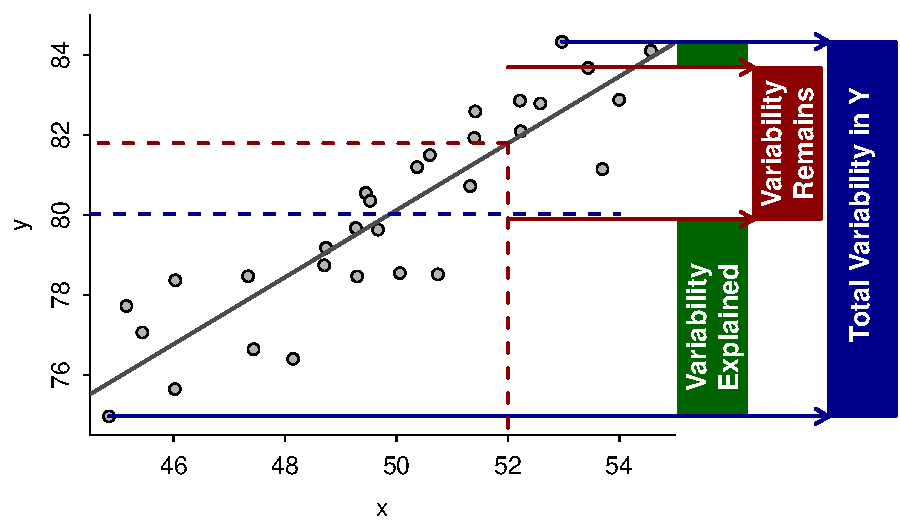
\includegraphics[width=.8\linewidth]{Figs/CoeffDeterm-1} 

}

\caption[Fitted line plot with visual representations of variabilities explained and unexplained]{Fitted line plot with visual representations of variabilities explained and unexplained. A full explanation is in the text.}\label{fig:CoeffDeterm}
\end{figure}


\end{knitrout}

Suppose now that the response variable is predicted for an individual with a known value of the explanatory variable (e.g., at the dashed vertical red line in \figref{fig:CoeffDeterm}). The predicted value for this individual is the value of the response variable at the corresponding point on the best-fit line (dashed horizontal red line). Again, because of natural variability, not all individuals with this value of the explanatory variable will have this exact value of the response variable. However, the prediction is now ``bracketed'' by the minimum and maximum value of the response variable \textbf{ONLY} for those individuals with the same value of the explanatory variable (solid red horizontal lines). Loosely speaking, this range is the ``variability in the response variable remaining after knowing the value of the explanatory variable'' (red box). This is the variability in the response variable that remains even after knowing the value of the explanatory variable or the variability in the response variable that cannot be explained away (by the explanatory variable).

The portion of the total variability in the response variable that was explained away consists of all the values of the response variable that would no longer be entertained as possible predictions once the value of the explanatory variable is known (green box in \figref{fig:CoeffDeterm}).

Now, by the definition of $r^{2}$, $r^{2}$ can be visualized as the area of the green box divided by the area of the blue box. This calculation does not depend on which value of the explanatory variable is chosen as long as the data are evenly distributed around the line (i.e., homoscedasticity -- see \sectref{sect:RegAssumptions}).

If the variability explained away (green box) approaches the total variability in the response variable (blue box), then $r^{2}$ approaches 1. This will happen only if the variability around the line approaches zero. In contrast, the variability explained (green box) will approach zero if the slope is zero (i.e., no relationship between the response and explanatory variables). Thus, values of $r^{2}$ also indicate the strength of the relationship; values near 1 are stronger than values near 0. Values near 1 also mean that predictions will be fairly accurate -- i.e., there is little variability remaining after knowing the explanatory variable.

\warn{A value of $r^{2}$ near 1 represents a strong relationship between the response and explanatory variables that will lead to accurate predictions.}


\section{Examples}
There are twelve questions that are commonly asked about linear regression results. These twelve questions are listed below with some hints about things to remember when answering some of the questions. An example of these questions in context is then provided.

\begin{enumerate}
  \item What is the response variable?  \textit{Identify which variable is to be predicted or explained, which variable is dependent on another variable, which would be hardest to measure, or which is on the y-axis.}
  \item What is the explanatory variable?  \textit{The remaining variable after identifying the response variable.}
  \item Comment on linearity and homoscedasticity. \textit{Examine fitted-line plot for curvature (i.e., non-linearity) or a funnel-shape (i.e., heteroscedasticity).}
  \item What is the equation of the best-fit line?  \textit{In the generic equation of the line ($y=mx+b$) replace $y$ with the name of the response variable, $x$ with the name of the explanatory variable, $m$ with the value of the slope, and $b$ with the value of the intercept.}
  \item Interpret the value of the slope. \textit{Comment on how the response variable changes by slope amount for each one unit change of the explanatory variable, on average.}
  \item Interpret the value of the intercept. \textit{Comment on how the response variable equals the intercept, on average, if the explanatory variable is zero.}
  \item Make a prediction given a value of the explanatory variable. \textit{Plug the given value of the explanatory variable into the equation of the best-fit line. Make sure that this is not an extrapolation.}
  \item Compute a residual given values of both the explanatory and response variables. \textit{Make a prediction (see previous question) and then subtract this value from the observed value of the response. Make sure that the prediction is not an extrapolation.}
  \item Identify an extrapolation in the context of a prediction problem. \textit{Examine the x-axis scale on the fitted-line plot and do not make predictions outside of the plotted range.}
  \item What is the proportion of variability in the response variable explained by knowing the value of the explanatory variable?  \textit{This is $r^{2}$.}
  \item What is the correlation coefficient?  \textit{This is the square root of $r^{2}$. Make sure to put a negative sign on the result if the slope is negative.}
  \item How much does the response variable change if the explanatory variable changes by X units?  \textit{This is an alternative to asking for an interpretation of the slope. If the explanatory variable changes by X units, then the response variable will change by X*slope units, on average.}
\end{enumerate}

All answers should refer to the variables of the problem -- thus, ``y'', ``x'', ``response'', or ``explanatory'' should not be in any part of any answer. The questions about the slope, intercept, and predictions need to explicitly identify that the answer is an ``average'' or ``on average.''

\warn{All interpretations should be ``in terms of the variables of the problem'' rather than the generic terms of x, y, response variable, and explanatory variable.}


\vspace{24pt}
\subsection*{Chimp Hunting Parties}
\begin{quote}
\textit{Stanford (1996) gathered data to determine if the size of the hunting party (number of individuals hunting together) affected the hunting success of the party (percent of hunts that resulted in a kill) for wild chimpanzees (Pan troglodytes) at Gombe. The results of their analysis for 17 hunting parties is shown in the figure below.\footnote{These data are in \href{https://raw.githubusercontent.com/droglenc/NCData/master/Chimp.csv}{Chimp.csv}.}  Use these results to answer the questions below.}
\end{quote}

\begin{knitrout}
\definecolor{shadecolor}{rgb}{0.922, 0.922, 0.922}\color{fgcolor}

{\centering 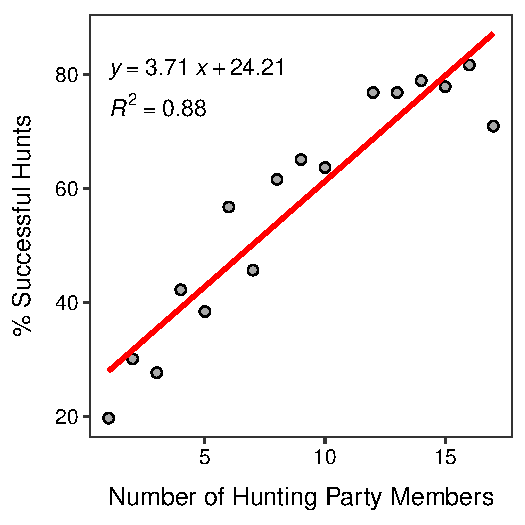
\includegraphics[width=.4\linewidth]{Figs/ChimpFLP-1} 

}



\end{knitrout}

\begin{QAlist}
  \item What is the response variable?
  \begin{QAlist}
    \item The response variable is the percent of successful hunts because the authors are attempting to see if success depends on hunting party size. Additionally, the percent of successful hunts is shown on the y-axis.
  \end{QAlist}
  \item What is the explanatory variable?
  \begin{QAlist}
    \item The explanatory variable is the size of the hunting party.
  \end{QAlist}
  \item Does any aspect of this regression concern you (i.e., consider the regression assumptions)?
  \begin{QAlist}
    \item The data appear to be very slightly curved but there is no evidence of a funnel-shape. Thus, the data may be slightly non-linear but they appear homoscedastic.
  \end{QAlist}
  \item In terms of the variables of the problem, what is the equation of the best-fit line?
  \begin{QAlist}
    \item The equation of the best-fit line is \% Success of Hunt = 24.21 + 3.71*Number of Hunting Party Members.
  \end{QAlist}
  \item Interpret the value of the slope in terms of the variables of the problem.
  \begin{QAlist}
    \item The slope indicates that the percent of successful hunts increases by 3.71, on average, for every increase of one member to the hunting party.
  \end{QAlist}
  \item Interpret the value of the intercept in terms of the variables of the problem.
  \begin{QAlist}
    \item The intercept indicates that the percent of successful hunts is 24.21, on average, for hunting parties with no members. This is nonsensical because 0 hunting members is an extrapolation.
  \end{QAlist}
  \item What is the predicted hunt success if the hunting party consists of 20 chimpanzees?
  \begin{QAlist}
    \item The predicted hunt success for parties with 20 individuals is an extrapolation, because 20 is outside the range of number of members observed on the x-axis of the fitted-line plot.
  \end{QAlist}
  \item What is the predicted hunt success if the hunting party consists of 12 chimpanzees?
  \begin{QAlist}
    \item The predicted hunt success for parties with 12 individuals is 24.21 + 3.71*12 = 68.7\%.
  \end{QAlist}
  \item What is the residual if the hunt success for 10 individuals is 50\%?
  \begin{QAlist}
    \item The residual in this case is $50$-(24.21 + 3.71*10) = $50$-61.3 = -11.3. Therefore, it appears that the success of this hunting party is 11.3\% lower than average for this size of hunting party.
  \end{QAlist}
  \item What proportion of the variability in hunting success is explained by knowing the size of the hunting party?
  \begin{QAlist}
    \item The proportion of the variability in hunting success that is explained by knowing the size of the hunting party is $r^{2}$=0.88.
  \end{QAlist}
  \item What is the correlation between hunting success and size of hunting party?
  \begin{QAlist}
    \item The correlation between hunting success and size of hunting party is $r=$0.94. [\emph{Note that this is the square root of $r^{2}$.}]
  \end{QAlist}
  \item How much does hunt success decrease, on average, if there are two fewer individuals in the party?
  \begin{QAlist}
    \item If the hunting party has two fewer members, then the hunting success would decrease by 7.4\% (i.e., $-2$*3.71), on average. [\emph{Note that this is two times the slope, with a negative as it asks about ``fewer'' members.}]
  \end{QAlist}
\end{QAlist}


\subsection*{Car Weight and MPG}
In \modref{chap:BivEDAQuant}, an EDA for the relationship between \var{HMPG} (the highway miles per gallon) and \var{Weight} (lbs) of 93 cars from the 1993 model year was performed. This relationship will be explored further here as an example of a complete regression analysis. In this analysis, the regression output will be examined within the context of answering the twelve typical questions. The results are shown in \figref{fig:CarFit}.

\begin{knitrout}
\definecolor{shadecolor}{rgb}{0.922, 0.922, 0.922}\color{fgcolor}\begin{figure}[h]

{\centering 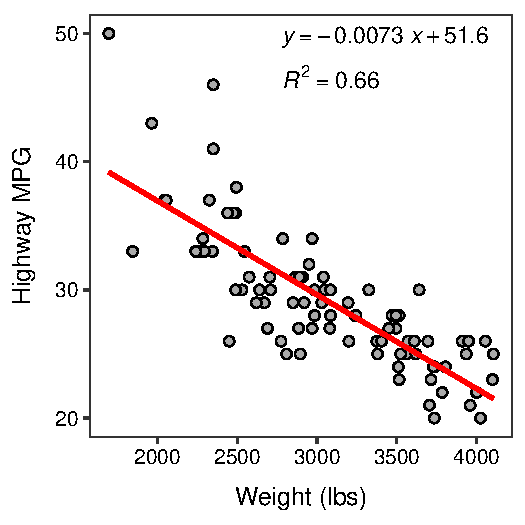
\includegraphics[width=.4\linewidth]{Figs/CarFit-1} 

}

\caption[Fitted line plot of the regression of highway MPG on weight of 93 cars from 1993]{Fitted line plot of the regression of highway MPG on weight of 93 cars from 1993.}\label{fig:CarFit}
\end{figure}


\end{knitrout}

\begin{QAlist}
  \item What is the response variable?
  \begin{QAlist}
    \item The response variable in this analysis is the highway MPG, because that is the variable that we are trying to learn about or explain the variability of.
  \end{QAlist}
  \item What is the explanatory variable?
  \begin{QAlist}
    \item The explanatory variable in this analysis is the weight of the car (by process of elimination).
  \end{QAlist}
  \item Do any aspects of this regression fit concern you?
  \begin{QAlist}
    \item The simple linear regression model appears to fit the data moderately well as the fitted-line plot \figrefp{fig:CarFit} shows only a very slight curvature and only very slight heteroscedasticity.\footnote{In advanced statistics books, objective measures for determining whether there is significant curvature or heteroscedasticity in the data are used. In this book, we will only be concerned with whether there is strong evidence of curvature or heteroscedasticity. There does not seem to be either here.}.
  \end{QAlist}
  \item In terms of the variables of the problem, what is the equation of the best-fit line?
  \begin{QAlist}
    \item The equation of the best-fit line for this problem is HMPG = 51.6 - 0.0073Weight.
  \end{QAlist}
  \item Interpret the value of the slope in terms of the variables of the problem.
  \begin{QAlist}
    \item The slope indicates that for every increase of one pound of car weight the highway MPG decreases by 0.0073, on average.
  \end{QAlist}
  \item Interpret the value of the intercept in terms of the variables of the problem.
  \begin{QAlist}
    \item The intercept indicates that a car with 0 weight will have a highway MPG value of 51.6, on average. [\emph{Note that this is the correct interpretation of the intercept. However, it is nonsensical because it is an extrapolation; i.e., no car will weigh 0 pounds.}]
  \end{QAlist}
  \item What is the predicted highway MPG for a car that weighs 3100 lbs?
  \begin{QAlist}
    \item The predicted highway MPG for a car that weighs 3100 lbs is 51.6 - 0.0073(3100) = 29.0 MPG.
  \end{QAlist}
  \item What is the predicted highway MPG for a car that weighs 5100 lbs?
  \begin{QAlist}
    \item The predicted highway MPG for a car that weighs 5100 lbs should not be computed with the results of this regression, because 5100 lbs is outside the domain of the data \figrefp{fig:CarFit}.
  \end{QAlist}
  \item What is the residual for a car that weights 3500 lbs and has a highway MPG of 24?
  \begin{QAlist}
    \item The predicted highway MPG for a car that weighs 3500 lbs is 51.6 - 0.0073(3500) = 26.1. Thus, the residual for this car is 24 - 26.1 = -2.1. Therefore, it appears that this car gets 2.5 MPG LESS than an average car with the same weight.
  \end{QAlist}
  \item What proportion of the variability in highway MPG is explained by knowing the weight of the car?
  \begin{QAlist}
    \item The proportion of the variability in highway MPG that is explained by knowing the weight of the car is $r^{2}$=0.66.
  \end{QAlist}
  \item What is the correlation between highway MPG and car weight?
  \begin{QAlist}
    \item The correlation between highway MPG and car weight is $r=$-0.81. [\emph{Not that this is the square root of $r^{2}$, but as a negative because form of the relationship between highway MPG and weight is negative.}
  \end{QAlist}
  \item How much is the highway MPG expected to change if a car is 1000 lbs heavier?
  \begin{QAlist}
    \item If the car was 1000 lbs heavier, you would expect the car's highway MPG to decrease by 7.33. [\emph{Note that this is 1000 slopes.}]
  \end{QAlist}
\end{QAlist}













%    \cleardoublepage
%    \phantomsection
%    \addcontentsline{toc}{part}{Appendix}
%    \chapter*{Appendices}
%    \appendix


%  \backmatter
%    %BIBLIOGRAPHY ---------------------------------------------------------------------------------------------------------
\cleardoublepage                             %not sure why but this is needed so TOC entry will point to right start page
\phantomsection                              %not sure why but this is needed so TOC entry will point to right start page
\addcontentsline{toc}{part}{Bibliography}    %Add a TOC entry
\bibliography{c:/aaaWork/zGnrlLatex/DHO_Bib} %make the bibliography
 
%INDEX ----------------------------------------------------------------------------------------------------------------
% cross references for the index
\index{Alternative Hypothesis|see{Hypothesis, Alternative}}
\index{Coefficient of Determination|see{$r^{2}$}}
\index{Forward calculation|see{Normal Distribution, Finding areas}}
\index{Frequency Table|see{Table, Frequency}}
\index{Goodness-of-Fit Test|see{Chi-square}}
\index{Line!Finding best-fit|see{Regression}}
\index{Mean!Inference|see{Z-test and t-Test}}
\index{Null Hypothesis|see{Hypothesis, Null}}
\index{Percentage Table|see{Table}}
\index{Proportions Table|see{Table, Proportion}}
\index{Row Proportions Table|see{Table, Proportion}}
\index{Column Proportions Table|see{Table, Proportion}}
\index{Table Proportions Table|see{Table, Proportion}}
\index{Proportions, Inference|see{Chi-square}}
\index{Rejection Criterion|see{$\alpha$}}
\index{Reverse calculation|see{Normal Distribution, Finding values}}
\index{Simple Linear Regression|see{Regression}}
\index{SLR|see{Regression}}
\index{Standard Normal Distribution|see{Normal Distribution}}
\index{Standardization|see{Normal Distribution, Converting to Z-scale}}
\index{One-sample Z-Test|see{Z-Test}}
\index{1-sample Z-Test|see{Z-Test}}
\index{One-sample t-Test|see{t-Test}}
\index{1-sample t-Test|see{t-Test}}
\index{Two-sample t-Test|see{t-Test}}
\index{2-sample t-Test|see{t-Test}}
\index{Matched-Pairs t-Test|see{t-Test}}
\index{Two-way Table|see{Table, Frequency}}
\index{Type I Error|see{Hypothesis Testing, Errors}}
\index{Type II Error|see{Hypothesis Testing, Errors}}
\index{Variability!Natural|see{Natural Variability}}
\index{Variability!Sampling|see{Sampling Variability}}
\index{Variable!Types|see{Quantitative, Continuous, Discrete, Categorical, Nominal, or Ordinal}}
\index{Variance!Testing Equality|see{Levene's Test}}
\index{Y-intercept|see{Intercept}}
\index{Z-Distribution|see{Normal Distribution, Standard Normal}}

% code to actually add the index
\addtocontents{toc}{\setlength{\cftbeforepartskip}{0.4em}}  %decrease dist before parts in back matter portion of TOC
\cleardoublepage                          %not sure why but this is needed so TOC entry will point to right start page
\phantomsection                           %not sure why but this is needed so TOC entry will point to right start page
\addcontentsline{toc}{part}{Index}        %Add a TOC entry
\printindex                               %Make the index


\end{document}
